\documentclass[border=10pt,tikz,multi]{standalone}
% \usetikzlibrary{shapes.geometric, positioning, arrows.meta}
\usetikzlibrary{positioning,shadows,arrows.meta,trees,shapes,fit}
\usetikzlibrary{graphs, graphs.standard, quotes}
\usepackage{fullpage}
\usepackage{calc}

\begin{document}

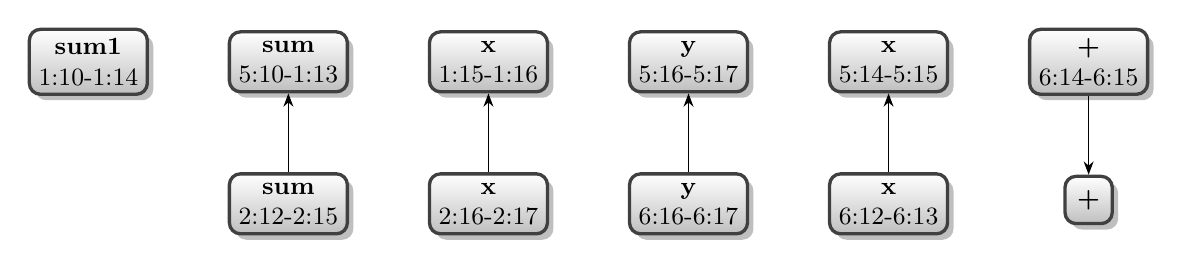
\begin{tikzpicture}
[font=\small, edge from parent,
    ->, >=Stealth,
    every node/.style={top color=white, bottom color=black!25,
    rectangle,rounded corners, minimum size=6mm, draw=black!75,
    very thick, drop shadow, align=center},
    edge from parent/.style={draw=black!50,thick},
    % level 1/.style={sibling distance=8cm},
    % level 2/.style={sibling distance=4cm},
    % level 3/.style={sibling distance=3cm},
    % level distance=1.5cm,
    ]

    \node (sum1) {\textbf{sum1} \\ 1:10-1:14};
    \node (sum) [right=of sum1] {\textbf{sum} \\ 5:10-1:13};
    \node (x1) [right=of sum] {\textbf{x} \\ 1:15-1:16};
    \node (y1) [right=of x1] {\textbf{y} \\ 5:16-5:17};
    \node (x2) [right=of y1] {\textbf{x} \\ 5:14-5:15};
    \node (plus_usage) [right=of x2] {\textbf{+} \\ 6:14-6:15};
    \node (plus) [below=of plus_usage] {\textbf{+}};

    \node (sum_usage) [below=of sum] {\textbf{sum} \\ 2:12-2:15};
    \node (x1_usage) [below=of x1] {\textbf{x} \\ 2:16-2:17};
    \node (y1_usage) [below=of y1] {\textbf{y} \\ 6:16-6:17};
    \node (x2_usage) [below=of x2] {\textbf{x} \\ 6:12-6:13};


    \draw (sum_usage) -- (sum);
    \draw (plus_usage) -- (plus);
    \draw (x1_usage) -- (x1);
    \draw (y1_usage) -- (y1);
    \draw (x2_usage) -- (x2);

\end{tikzpicture}

\end{document}


